\documentclass[12pt]{article}

%-------------PACKAGES------------- 
\usepackage[margin=1in]{geometry} 
\usepackage{amsmath,amsthm,amssymb}
\usepackage{pgfplots}
\usepackage{float}
\usepackage{braket}
\usepackage{titling}
\usepackage{tikz}
\usepackage{mathtools}
\usepackage{listings}
\usepackage{color}
\usepackage{caption}
\usepackage{subcaption}
\usepackage{algorithm,algpseudocode}

%-------------FORMATTING-------------
\setlength{\droptitle}{-6em} 
\setlength{\parindent}{0pt}
 
%--------------COMMANDS--------------
\newcommand{\N}{\mathbb{N}}
\newcommand{\Z}{\mathbb{Z}}
\newcommand{\R}{\mathbb{R}}
\newcommand{\C}{\mathbb{C}}
%\renewcommand{\qedsymbol}{\filledbox}

\DeclarePairedDelimiter \abs{\lvert}{\rvert}%
\DeclarePairedDelimiter \babs{\bigg\lvert}{\bigg\rvert}%
\DeclarePairedDelimiter \norm{\lVert}{\rVert}%

%------------ENVIRONMENTS------------- 
\newenvironment{theorem}[2][]{\begin{trivlist}
\item[{\bfseries #1}\hskip \labelsep {\bfseries #2.}]}{\end{trivlist}}
\newenvironment{lemma}[2][Lemma]{\begin{trivlist}
\item[\hskip \labelsep {\bfseries #1}\hskip \labelsep {\bfseries #2.}]}{\end{trivlist}}
\newenvironment{exercise}[2][Exercise]{\begin{trivlist}
\item[\hskip \labelsep {\bfseries #1}\hskip \labelsep {\bfseries #2.}]}{\end{trivlist}}
\newenvironment{reflection}[2][Reflection]{\begin{trivlist}
\item[\hskip \labelsep {\bfseries #1}\hskip \labelsep {\bfseries #2.}]}{\end{trivlist}}
\newenvironment{proposition}[2][Proposition]{\begin{trivlist}
\item[\hskip \labelsep {\bfseries #1}\hskip \labelsep {\bfseries #2.}]}{\end{trivlist}}
\newenvironment{corollary}[2][Corollary]{\begin{trivlist}
\item[\hskip \labelsep {\bfseries #1}\hskip \labelsep {\bfseries #2.}]}{\end{trivlist}}
\theoremstyle{remark}
\newtheorem*{remark}{Remark}

%-------------CODE-STYLE------------
\definecolor{dkgreen}{rgb}{0,0.6,0}
\definecolor{gray}{rgb}{0.5,0.5,0.5}
\definecolor{mauve}{rgb}{0.58,0,0.82}
\lstset{frame=tb,
	language=C++,
	aboveskip=3mm,
	belowskip=3mm,
	showstringspaces=false,
	columns=flexible,
	basicstyle={\small\ttfamily},
	numbers=none,
	numberstyle=\tiny\color{gray},
	keywordstyle=\color{blue},
	commentstyle=\color{dkgreen},
	stringstyle=\color{mauve},
	breaklines=true,
	breakatwhitespace=true,
	tabsize=3
}

\lstset{
	morekeywords={end}
}

%------------------------------------ 
%---------START-OF-DOCUMENT----------
%------------------------------------

\begin{document}
 
\title{Homework 10}
\author{David Miller \\ 
MAP5345: Partial Differential Equations I} 
 
\maketitle

\section*{Problem 1}

\textit{Prove the identity}
\begin{align}
	\nabla \cdot (u\nabla v - v\nabla u) = u \Delta v - v\Delta u
\end{align}
\textit{for any two functions $u(x,y,z)$ and $v(x,y,z)$ that are are sufficiently smooth.} \\

Lets have a bit more fun and assume that $u$ and $v$ are in $\R^d$. Then we have 

\begin{align*}
	\nabla \cdot (u\nabla v - v\nabla u) & = \nabla \cdot \bigg(u\sum\limits_{i=1}^d\frac{\partial v}{\partial x_i}\hat{e}_i - v\sum\limits_{i=1}^d\frac{\partial u}{\partial x_i}\hat{e}_i\bigg) 
	\\ & = \nabla \cdot \bigg( \sum\limits_{i=1}^du\frac{\partial v}{\partial x_i}\hat{e}_i \bigg) - \nabla \cdot \bigg( \sum\limits_{i=1}^dv\frac{\partial u}{\partial x_i}\hat{e}_i \bigg)
	\\ & = \sum\limits_{i=1}^d\frac{\partial}{\partial x_i}\bigg(u\frac{\partial v}{\partial x_i}\hat{e}_i\bigg) - \sum\limits_{i=1}^d\frac{\partial}{\partial x_i}\bigg(v\frac{\partial u}{\partial x_i}\hat{e}_i\bigg) 
	\\ & = \sum\limits_{i=1}^d \bigg(u\frac{\partial^2v}{\partial x_i^2} + \frac{\partial u}{\partial x_i}\frac{\partial v}{\partial x_i}\bigg)\hat{e_i} - \sum\limits_{i=1}^d \bigg(v\frac{\partial^2u}{\partial x_i^2} + \frac{\partial u}{\partial x_i}\frac{\partial v}{\partial x_i}\bigg)\hat{e_i}
	\\ & = u\sum\limits_{i=1}^d \frac{\partial^2v}{\partial x_i^2} - v\sum\limits_{i=1}^d\frac{\partial^2u}{\partial x_i^2}\hat{e_i}
	\\ & = u\Delta v - v\Delta u
\end{align*}
where this holds true for $d = 3$.

\newpage

\section*{Problem 2}

\textit{Consider (vanishing) Robin boundary conditions in three spatial dimensions}
\begin{align}
	au + b\frac{\partial u}{\partial n} = 0, \quad \text{for } x,y,z \in \partial\Omega
\end{align} 

\textit{for some real constants $a$ and $b$.} \\

\textit{a) Prove that these boundary conditions are symmetric.} \\

To prove symmetric boundary conditions we must show
\begin{align*}
	\int_{\partial\Omega} u\frac{\partial v}{\partial n} - v\frac{\partial u}{\partial n} \, ds = 0
\end{align*}
for all $u$ and $v$ that satisfy the boundary conditions (2). From (2) we have that 
\begin{align*}
	u = -\frac{b}{a}\frac{\partial u}{\partial n}, \quad v = -\frac{b}{a}\frac{\partial v}{\partial n}
\end{align*}
where $a \neq 0$ (this would be vanishing Neumann BC) and $b \neq 0$ (this would be vanishing Dirichlet BC). Plugging this in we get
\begin{align*}
	\int_{\partial\Omega} u\frac{\partial v}{\partial n} - v\frac{\partial u}{\partial n} \, ds = -\frac{b}{a}\int_{\partial \Omega}\frac{\partial u}{\partial n}\frac{\partial v}{\partial n} - \frac{\partial u}{\partial n}\frac{\partial v}{\partial n} \, ds = 0
\end{align*}
thus showing vanishing Robin BCs are symmetric. \\

\textit{b) What if $a$ and $b$ are not constants, but variable coefficients, $a(x,y,z), b(x,y,z)$? Are the boundary conditions still symmetric? If so, prove it.} \\

The coefficients $a(x,y,z)$ and $b(x,y,z)$ must sill satisfy (2) so we can still arrive at the same conclusions as we did in part (a). If either $a(x,y,z)$ or $b(x,y,z)$ is equal to 0 then the BCs just collapse to Neumann or Dirichlet BCs and are still symmetric. \\

\textit{c) Now consider the Laplacian operator with the above vanishing Robin boundary conditions. Now that you know the conditions are symmetric, what can you say about the eigenvalues and eigenfunctions fo the Laplacian?} \\

The Laplacian operation is then self-adjoint. It follows from our Big Theorem that 
\begin{enumerate}
	\item The eigenvalues are real
	\item The eigenfunctions with distinct eigenvalues are orthogonal 
	\item If there are repeated eigenvalues then the corresponding eigenfunctions can be made orthogonal
\end{enumerate}

\newpage

\section*{Problem 3}

\textit{Consider heat conduction of temperature $u(x,y,z)$ on the unit square $\Omega = \{(x,y)$ such that $0 < x < 1$ and $0 < y < 1\}$, with the following mixed boundary conditions}
\begin{align}
	& u_t = k\Delta u \quad \text{for }(x,y) \in \Omega \\
	& u_x = 0 \quad \text{for } x = 0,1 \\
	& u = 0 \quad \text{for } y = 0,1 \\
	& u(x,y,0) = u_0(x,y)
\end{align}
\textit{a) Find the general solution to the IBVP.} \\

Assume the solution takes on the form $u(x,y,t) = X(x)Y(y)T(t)$. Plugging this into (3) gets us
\begin{align*}
	XYT^\prime & = kX^{\prime\prime}YT + kXY^{\prime\prime}T \\
	\Rightarrow \quad \frac{T^\prime}{kT} & = \frac{X^{\prime\prime}}{X} + \frac{Y^{\prime\prime}}{Y}
\end{align*}
The only way the LHS can be equal to the RHS is if they both equal some constant. Therefore let $X^{\prime\prime}/X = -A, \, Y^{\prime\prime}/Y = -B, \,$ and $T^\prime/kT = -A - B$. From this we get 
\begin{align*}
	X & = C_1\cos(\sqrt{A}x) + C_2\sin(\sqrt{A}x) \\
	Y & = C_3\cos(\sqrt{B}x) + C_4\sin(\sqrt{B}x) \\
	T & = e^{-k(A+B)t}
\end{align*}
Using the boundary conditions yields $C_2 = C_3 = 0$ and $A = m^2\pi^2$, $B = n^2\pi^2$. The general solution is then 
\begin{align*}
	u(x,y,t) = \sum\limits_{m=0}^\infty\sum\limits_{n=1}^\infty A_{nm} \cos(m\pi x)\sin(n\pi y) e^{-k\pi^2(n^2 + m^2)t}
\end{align*}

\textit{b) Note that there are several repeated eigenvalues. Show explicitly that the eigenfunctions you found are already orthogonal. Hence, there is no need to perform Gram Schmidt.} \\ 

\begin{align*}
\braket{X_mY_n, X_{m^\prime}Y_{n^\prime}} & = \int\limits_0^1\int\limits_0^1 \cos(m\pi x)\sin(n\pi y)\cos(m^\prime \pi x)\sin(n^\prime \pi y) \, dxdy
\\ & = \int\limits_0^1 \cos(m\pi x)\cos(m^\prime\pi x) \, dx \int\limits_0^1 \sin(n\pi y)sin(n^\prime\pi y) \, dy 
\\ & = -\frac{1}{16}\int\limits_0^1 (e^{im\pi x} + e^{-im\pi x})( e^{im^\prime\pi  x} + e^{-im^\prime\pi  x}) \, dx \int\limits_0^1 (e^{in\pi y} - e^{-in\pi y})( e^{in^\prime\pi  y} - e^{-in^\prime\pi  y}) \, dy 
\\ & = -\frac{1}{16}\int\limits_0^1 e^{i(m+m^\prime)\pi  x} + e^{-i(m+m^\prime)\pi  x} + e^{i(m-m^\prime)\pi x} + e^{i(m^\prime-m)\pi x} \, dx 
\\ & \times \int\limits_0^1 e^{i(n+n^\prime)\pi y} + e^{-i(n+n^\prime)\pi y} - e^{i(n-n^\prime)\pi y} - e^{i(n^\prime-n)\pi y} \, dy 
\\ & = -\frac{1}{4}\int\limits_0^1 \cos((m+m^\prime)\pi x) + \cos((m-m^\prime)\pi x) \, dx \int\limits_0^1 \cos((n+n^\prime)\pi y) - \cos((n-n^\prime)\pi y) \, dy
\\ & = -\frac{1}{4}\bigg(\frac{\sin((m+m^\prime)\pi x)}{(m+m^\prime)\pi} + \frac{\sin((m-m^\prime)\pi x)}{(m-m^\prime)\pi}\bigg)\bigg(\frac{\sin((n+n^\prime)\pi y)}{(n+n^\prime)\pi} - \frac{\sin((n-n^\prime)\pi y)}{(n-n^\prime)\pi}\bigg)\bigg\vert_0^1\bigg\vert_0^1
\\ & = 0
\\
\\ \braket{X_mY_n,X_mY_n} & = \int\limits_0^1\int\limits_0^1 \cos^2(m\pi x)\sin^2(n\pi y) \, dxdy
\\ & = -\frac{1}{16}\int\limits_0^1 \bigg(e^{in\pi x} + e^{-in\pi x}\bigg)^2 \, dx\int\limits_0^1 \bigg(e^{im\pi y} - e^{-im\pi y}\bigg)^2 \, dy
\\ & = -\frac{1}{16}\int\limits_0^1 e^{2in\pi x} + e^{-2in\pi x} + 2 \, dx \int\limits_0^1 e^{2im\pi y} + e^{-2im\pi y} - 2 \, dy 
\\ & = -\frac{1}{4}\int\limits_0^1 \cos(2m\pi x) + 1 \, dx\int\limits_0^1 \cos(2n\pi y) - 1 \, dy
\\ & = -\frac{1}{4}\bigg(\frac{\sin(m\pi x)\sin(n\pi y)}{4mn\pi^2} - \frac{sin(2m\pi x)}{2m\pi}y + \frac{sin(2n\pi y)}{2n\pi}x - xy  \bigg)\bigg\vert_0^1\bigg\vert_0^1
\\ & = \frac{1}{4}
\end{align*}
Therefore there is no need to perform Gram Schmidt.

\textit{c) Set $k = 5$ and consider the initial condition $u_0(x,y) = y - y^2$. Use projection to determine the coefficients in your general solution.} \\

\begin{align*}
	A_{mn} & = \frac{\braket{u_o,X_mX_n}}{\braket{X_mX_n,X_mX_n}}
	\\ & = 4\int\limits_0^L \int\limits_0^L (y-y^2)\sin(n\pi y)\cos(m\pi x) \, dxdy 
	\\ & = 4\int\limits_0^L \cos(m\pi x) \, dx \int\limits_0^1 (y-y^2)\sin(n\pi y) \, dy
	\\ & = 4\int\limits_0^1 (y - y^2)\sin(n\pi y) \, dy \tag{$m=0$} 
	\\ & = \frac{16}{n^3\pi^3} \text{, \quad for $n$ odd} \tag{see HW 2} 
\end{align*}
Therefore we have the solution
\begin{align*}
	u(x,y,t) = \sum\limits_{n=1}^\infty \frac{16}{(2n-1)^3\pi^3}\sin((n-1)\pi y)e^{-5(2n-1)^2\pi^2t}
\end{align*}

\textit{d) Using Julia, plot the solution at a few different time values. This will require 2D plots and I recommend making contour plots.} 


\newpage

\begin{figure}[h]
	\centering
	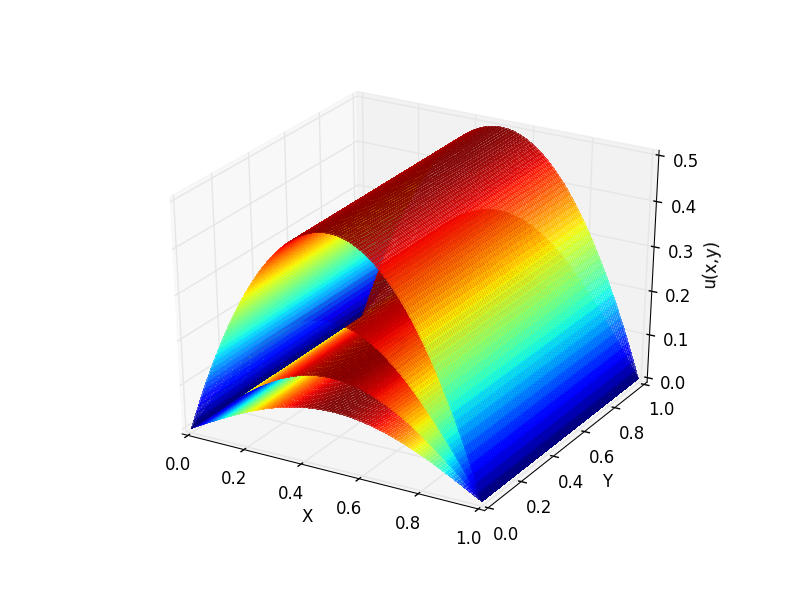
\includegraphics[width=15cm]{figure_1.png}
	\caption{2D Heat Equation}
\end{figure}

\end{document}